% Формат дипломной работы:
%     - шрифт 14
%     - бумага А4
%     - поля 2х2х2х2см
%     - полуторный межстрочный интервал
\documentclass[14pt]{extarticle}
\usepackage[paper=a4paper, top=2cm, bottom=2cm, right=1cm, left=3cm]{geometry}
\linespread{1.3}

% Стиль оглавления
\usepackage{titletoc}
\titlecontents{section}[2em]{\bfseries\addvspace{0.5em}}
{\contentslabel[\thecontentslabel]{1.7em}}
{}{\titlerule*[1pc]{.}\contentspage}

\usepackage[utf8]{inputenc}                % Кодировка
\usepackage[T1,T2A]{fontenc}
\usepackage[main=russian, english]{babel}  % Русский язык
\usepackage[pdftex]{graphicx}              % Картинки
\usepackage{indentfirst}                   % Отступ перед абзацами

\usepackage[unicode]{hyperref}                                         % Ссылки и русские закладки
\hypersetup{                                                          %
    pdftitle={Курсовая работа},                                        % Название документа
    pdfsubject={Параллельное что-то},                                  % Тема документа
    pdfauthor={Егоров Кирилл Юлианович},                               % Автор документа
    pdfcreator={Кафедра системного анализа ВМК МГУ},                   % Создатель документа
    pdfproducer={LaTeX},                                               % Программа, создавшая документ
    hidelinks                                                          % Скрывает рамку вокруг ссылок
}

\usepackage{amsfonts}
\usepackage{amssymb}
\usepackage{amsmath}

\begin{document}
    \thispagestyle{empty}
\begin{center}
    \ \vspace{-3cm}

    
\includegraphics[width=0.5\textwidth]{title_page/msu.eps}\\

    {\small{\scshape  Московский государственный университет имени М.~В.~Ломоносова}\\
    Факультет вычислительной математики и кибернетики\\
    Кафедра системного анализа}

    \vfill

    {\Large Егоров Кирилл Юлианович}

    \vspace{1cm}

    {\LARGE\bfseries Построение параллельных алгоритмов для решения задачи быстродействия с фазовыми ограничениями}

    \vspace{1.5cm}

    {\scshape Курсовая работа}
\end{center}

\vspace{3cm}

\begin{flushright}
    \large
    \textit{Научный руководитель}\\
    к.ф.-м.н., доцент И.~В.~Востриков
\end{flushright}

\vfill

\begin{center}
    Москва, 2022
\end{center}

\clearpage
    \tableofcontents
    \clearpage

    \section{Введение}
    Работа посвящена разработке параллельных алгоритмов для поиска оптимального по быстродействию пути между двумя точками на некоторой ограниченной территории с препядствиями, которые мешают движению.
В~работе эти препядствия представляют собой произвольные области, в которых невозможно дальнейшее движение.

Для представления в виде классической \textit{задачи кратчайшего пути} исходная задача дискретизуются.
Численное решение уравнения Гамильтона--Якоби--Беллмана, к которому сводится непрерывный вариант возможно
 (по крайней мере, в \cite{gyb} предложен способ решения после нескольких приближений и дискретизации уравнения), но дискретизация задачи в целом~--- более популярное решение. 

Необходимость решения задачи кратчайшего пути в двумерном пространстве возникает в различных сферах, но в первую очередь в транспортной и логистической.
Сложно представить будущее, где проблема быстрой доставки товаров или безопасного перемещения людей перестала быть актуальной.
Данная задача является классической и традиционно решается методом динамического программирования\cite{bellman}.

Последовательные алгоритмы, решающие данную задачу хорошо изучены и представлены в статьях \cite{dijkstra} и \cite{review}.
Эти алгоритмы были адаптированы под поставленную задачу, и на их основе были разработаны параллельные варианты.

Было уделено вниманию различным способам организации параллелелизма: на многоядерном процессоре, на графическом процессоре, на многонодной компьютерной установке.
Для каждого способа описан соответствующий алгоритм, для двух видов параллелелизма разработаны программы и замерены времена работы.
    \newpage
    \section{Постановка задачи}
    Рассмотрим управляемый объект, положение которого задается динамической системой дифференциальных уравнений
\begin{equation}\label{first}
    \frac{dx}{dt} = f(t, x, u)
\end{equation}
на промежутке $t_0 \leqslant t \leqslant t_1$ с заданным начальным состоянием $x(t_0) = x^0$.

Такое описание естесственно для движений, подчиняющихся второму закону Ньютона.
В нашем случае $x = [x_1, x_2, v_1, v_2]\in \mathbb{R}^4,\;v_i=\dot x_i,\,i=\{1,2\}$.
Наложим на фазовые координаты следующие ограничения:
\[
    [x_1, x_2] \in \Omega, \quad [v_1, v_2] \in \Omega_v.
\]

Для задачи Коши (\ref{first}) поставим задачу поиска управления $u \in U$, минимизирующего следующий интегральный функционал:
\begin{equation}
    J(u) = \int\limits_{t_0}^{t_1} g(x(t), u(t))\,dt \rightarrow \min\limits_{u\in U}.
\end{equation}

Будем пользоваться методом динамического программирования. Введем функцию цены
\[
    \begin{aligned}
        &V(t,x) = \min\limits_{u \in U}\int\limits_{t}^{t_1}g(x(t), u(t))\,dt,\\
        &V(t_1,x^1) = 0.
    \end{aligned}
\]
Согласно \cite{optcontrol}, если предполагать непрерывную дифференцируемость функции цены, решение задачи равносильно решению уравнения Гамильтона--Якоби--Беллмана:
\begin{equation}\label{gyb}
    \min\limits_{u(t) \in U}\left\{
        g(x,u) + \sum\limits_{i=1}^{n}\frac{\partial V(x)}{\partial x_i} f_i(x,u)
    \right\} = 0.
\end{equation}

\textit{Замечание.}
Мы рассматриваем частный случай этой задачи --- задачу быстродейсвия, то есть задачу с функционалом качества $g(x,u) \equiv 1$. В этих условиях уравнение Гамильтона--Якоби--Беллмана (\ref{gyb}) будет записано в следующем виде:
\[
    \min\limits_{u\in U}\langle \nabla t(x), f(x,u) \rangle = -1.
\]

Вместо дискретизации и последующего решения получившегося уравнения мы дискретизируем исходную задачу для приведения ее к виду задачи кратчайшего пути.

Пусть $\Pi$~--- минимальный прямоугольник, вмещающий в себя целиком множество $\Omega$. Введем на нем равномерную сетку с шагом $\varepsilon$:
\begin{equation}
    (i,j):\;1\leqslant i \leqslant N,\,1\leqslant i \leqslant M
\end{equation}
\begin{equation}
    \Xi = \left\{ (x_i , y_j) \in \Pi , x_i = \varepsilon\frac{i}{N} , y_j = \varepsilon\frac{j}{M} \right\}.
\end{equation}

Мы будем считать, что $x^0,x^1 \in \Xi$. Перемещение возможно только в ``соседние'' узлы сетки, содержащиеся в множестве фазового ограничения $\Omega$. Назовем такое множество \textit{возможным}:
\[
    \mathrm{possible}(i,j) = \{
        (i, j) \;|\; i \in \{i, i \pm 1\}, j \in \{j, j \pm 1\}, (x_i,y_j) \in \Omega    
    \}
\]

\textit{Предположение.} На каждом этапе пути можно ехать лишь с некоторой одной скоростью и скорость на предыдущем участке не влияет на время прохода следующего участка.

Данное предположение кажется резонным, если мы рассматриваем, например, автомобиль или человека, а шаг сетки~--- несколько десятков метров: такого расстояния должно хватить для изменения скорости на оптимальную для данного типа поверхности. Для объектов, не удовлетворяющих этому свойству, такое предположение не подходит. Предположение позволяет сократить размернось рассматриваемого фазового пространства с 4 до 2, но превращает управление в импульсное.

Тогда, мы можем считать известным время перехода между точкой $(i,j)$ и любой точкой из ее возможного множества:
\[
    d_{i,j}(\hat i, \hat j),\;\mbox{где $(\hat i, \hat j) \in \mathrm{possible}(i,j)$}.
\]

Таким образом, получили матричное уравнение в неявном виде, которое предстоит решить:
\begin{equation}
    \begin{aligned}
        &V_{i,j} = \min\limits_{(\hat i, \hat j) \in \mathrm{possible}(i, j)}\{d_{i,j}(\hat i,\hat j) + V_{\hat i, \hat j}\}, \\
        &V_{i_1, j_1} = 0.
    \end{aligned}
\end{equation}
    \section{Алгоритм Беллмана--Форда}
    Данный раздел содержит описание алгоритма Беллмана--Форда в применении к нашей задачи, а также в процессе описаны общие принципы работы построенных алгоритмов, которые будут использованы и в дальнейшем.

Традиционно для алгоритмов данного типа (алгоритм поиска кратчайшего пути) маркирование узлов сетки предполагаемым оптимальным значением функционала.
Маркировка одного и того же узла может происходить один или несколько раз, но в результате работы программы маркировки каждой вершины должны соответствовать оптимальному значению функционала качества для данной вершины.
Поэтому далее мы будем обозначать маркировку как $V(i, j)$, а перемаркирование как $V(i, j) \leftarrowtail v$.
Изначально предполагается, что все вершины, кроме целевой, имеют маркировку $+\infty$. Целевая же вершина $(i_1, j_1)$ имеет маркировку $0$.

Ниже приведено описание алгоритма:

\begin{enumerate}
    \item Необходимо провести $(NM - 1)$ итерации алгоритма.
    \item На каждой итерации происходит полный проход по сетке. Далее $(i,j)$ --- позиция при проходе.
    \item Для каждой вершины из возможного множества $(\hat i, \hat j) \in \mathrm{possible}(i,j)$ происходит перемаркировка: в случае, если $V(i, j) > d_{i,j}(\hat i, \hat j) + V(\hat i, \hat j)$, перемаркируем
    \[
        V(i,j) \leftarrowtail d_{i,j}(\hat i, \hat j) + V(\hat i, \hat j).
    \]
\end{enumerate}

Заметим, что оптимальная траектория не может иметь более $(NM - 1)$ перемещения. Таким образом алгоритм действительно ищет кратчайший путь.

\subsection{Распараллеливание на CPU}
Ядра центрального процессора~--- это высокопроизводительные процессоры, которые есть в каждом компьютере. В стандартном персональном компьютере от 4 до 16 ядер. Пусть на компьютере имеется $C$ ядер.

Предлагается распараллелить проход по сетке по переменной $i$. Разобьем сетку на $(C-1)$ штуку размером $\left\lfloor \frac{N}{C}\right\rfloor \times M$ и одну размера $N-(C-1)\left\lfloor \frac{N}{C} \right\rfloor \times M$. Каждое ядро должно обрабатывать собственную матрицу.

Возникающую проблему синхронизации процессов при обработке соседних подматриц предлагается решать массивом мьютексов~---примитивов синхронизации, обеспечивающих взаимное исключение исполнения критических участков кода.

Перед началом основной программы каждый мьютекс из массива $A$ размера $C$ переводится в закрытое состояние. По окончании обработки $c \in \{0,\ldots,C-1\}$ процессом первой строки процесс переводит мьютекс $A_{c}$ в открытое состояние. Перед началом обработки последней строки процесс $c$ дожидается открытия мьютекса $A_{c+1}$, если $c+1<C$.

\subsection{Распараллелевание на GPU}
Параллельные вычисления на графическом процессоре в последние годы очень активно развиваются. Это связано с типичной архитектурой таких процессоров: это большое количество маломощных процессоров с общей памятью. Почти всегда такие вычисления используются для майнинга криптовалюты.

На сегодняшний стандартной архитектурой для написания программ на GPU является CUDA SDK, поддерживаемая исключительно графическими картами компании Nvidia. Ввиду отсутствия данного графического процессора, мы ограничимся лишь описанием алгоритма, в сравнении времени работы программ данный алгоритм принимать участие не будет.

Предлагается вместо одного прохода по сетке на каждой итерации, проходить 8 раз (по числу максимальной мощности возможного множества). При этом каждый узел при таком проходе будет обработан параллельно. На каждом из восьми проходов будет обработано только одно возможное направление движения, причем у всех узлов оно должно совпадать. Таким образом мы обеспечиваем синхронизацию.

\subsection{Распараллеливание на многонодной установке}
Предлагается использовать модель \textit{master-follower}. Пусть имеется одна \textit{master} нода, с которой осуществляется оркестрация установки, и $L$ \textit{follower} нод с $C_l, l=\overline{1,L}$ доступных ядер процессора, используемых непосредственно для вычислений. Предполагается, что между нодами настроена сеть и известны адреса всех сервисов.

Программа поставляется в виде http-сервиса вычислителя, и основной программы, которая общается с вычислителями посредством http запросов. На \textit{follower} нодах запускаются сервисы вычислителя в количестве, соответствующим количеству доступных ядер процессора.

Параллелелизм осуществляется как и в случае распараллелевания на CPU. Но из-за отсутствия общей памяти возникает проблема синхронизации данных между всеми вычислителями. Для этого по результатам обработки основная программа должна передать вычислителям минимальное инкрементальное изменение состояния для данного вычислителя. Для этого последняя строка каждого батча считается основной программой еще один раз, после чего эта строка отправлется вычислителю для синхронизации.
    \section{Алгоритм Дейкстры}
    Алгоритму Дейкстры~--- это самый популярный алгоритм поиска кратчайшего пути. Из-за меньшей, чем у алгоритма Беллмана--Форда алгоритмической сложности, данный алгоритм позволяет производить вычисления на сетках на порядок большего размера. 

Алгоритм использует две дополнительные структуры: множество обработанных узлов и можество граничных узлов. Данные структуры имплементированы как хэш-таблицы.

Ниже приведено описание алгоритма:
\begin{enumerate}
    \item На начало алгоритма в множестве граничных узлов находится только целевой узел. 
    \item На каждой итерации алгоритма из множества граничных узлов выбирается узел с минимальной маркировкой.
    \item Этот узел добавляется в множество обработанных узлов и удаляется из граничного множества.
    \item Затем из возможного множества выбираются узлы, которые не находятся в множестве обработанных узлов. Эти узлы добавляются в множество граничных вершин, маркировка таких вершин обновляется.
\end{enumerate}
Алгоритм останавливается в случае, если на некоторой итерации алгоритма был выбран начальный узел $(i_0,j_0)$.

\subsection{Распараллелевание на CPU}

Основной затратной операцией в приведенном алгоритме является поиск минимума на каждой итерации.
Поэтому параллелелизм будет встроен именно в этот этап.

Для этого предлагается хранить граничное множество в $C$ хэш-таблицах.
Добавлять узел в наименее наполненную таблицу.
Тогда каждый процесс ищет минимум в своей хэш-таблице, а затем основной процесс ищет минимум в массиве из $C$ элементов.

\subsection{Распараллелевание на многонодной установке}

Для обеспечения синхронизации снова пользуемся инкрементальным обновлением.
Заметим, что за одну итерацию алгоритма происходит одно добавление в множество обработанных вершин, и не более 7 добавлений в граничное множество.
Этой информации достаточно для поддержания всех вычислителей в актуальном состоянии, поэтому она должна сообщаться сервисам-вычислителям после каждой проведенной итерации.
    \section{Описание программного решения}
    Программное решение представлено на языке \textit{Go}. Причины для использования этого языка при написании вычислительных параллельных задач следующие:
\begin{enumerate}
    \item Go --- компилируемый язык со встроенной сборкой мусора. Это необычное сочетание качеств колоссально повышает скорость разработки, при этом язык проигрывает в производительности языку C всего в 1,5--2 раза.
    \item Go представляет современные средства параллелелизма \textit{go routines}. В отличие от классических потоков (threads) рутины управляются не операционной системой, а \textit{go runtime}, за счет чего значительно сокращаются накладные расходы на создание таких рутин и на коммуникацию между ними.
\end{enumerate}

Помимо основных алгоритмов были написаны сопутствующие программы для генрации начальных данных и визуализации результатов. Генерация карты высот происходит посредством последовательного сложения нескольких шумов Перлина с подобранными различными параметрами для получения похожего на земной ландшафта \cite{perlin}. Карту с различными типами почв и фазовыми ограничениями предлагается самостоятельно нарисовать пользователю в любом графическом редакторе, например, Microsoft Paint, перед запуском программы.

В случае распрараллелевания на многонодной установке, программа поставляется в виде двух docker-образов и Ku\-ber\-ne\-tes манифестов для последовательного применения для деплоя на кластер, оркестрируемый Kubernetes. На других облачных оркестраторах решение не проверялось. Написание Ku\-ber\-ne\-tes оператора для данного решения видится нецелесообразным, ввиду отсутствия у программы сложного жизненного цикла.

Визуализация сделана с помощью платформо-независимой спецификации OpenGL, что позволяет собирать все компоненты под различные операционный системы. Ниже представлены несколько примеров работы программы. Все алгоритмы выдают одинаковый результат, однако всвязи с разной асимптотической сложностью, алгоритм Беллмана--Форда имеют размер сетки на порядок меньше, чем для алгоритма Дейстры.

В примерах ниже, время перехода принято равным
\[
    d_{i,j}(\hat i, \hat j) = 100\cdot(\mathrm{height}(\hat i, \hat j) - \mathrm{height}(i, j))_{+} + 5.
\]

\begin{figure}[h]
    \centering
    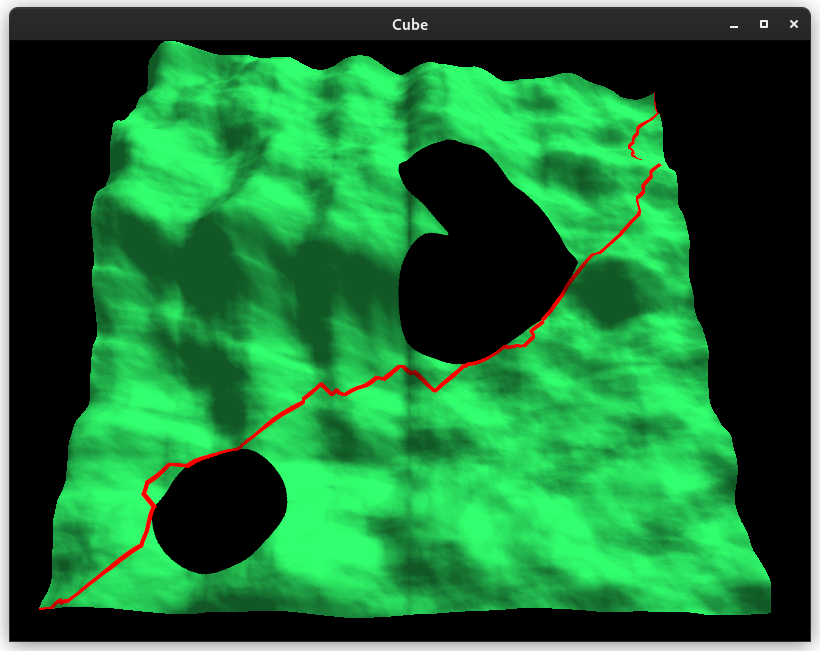
\includegraphics[scale=0.5]{content/dijkstra-top.png}
    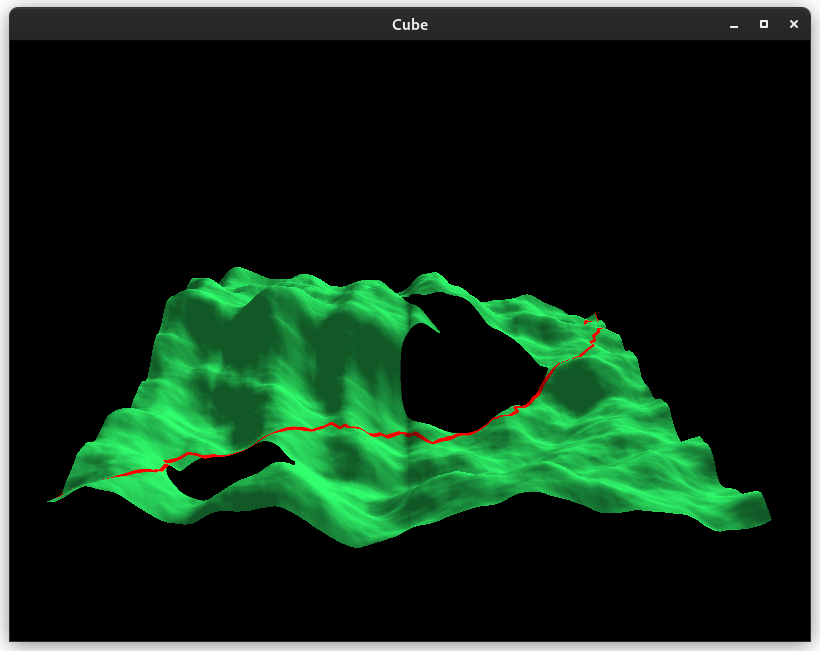
\includegraphics[scale=0.5]{content/dijkstra.png}
    \caption{Результат работы алгоритма Дейкстра на сетке 1000$\times$1000 c начальной позицией $(1, 1)$, конечной $(1000, 1000)$.}
\end{figure}

\begin{figure}[h]
    \centering
    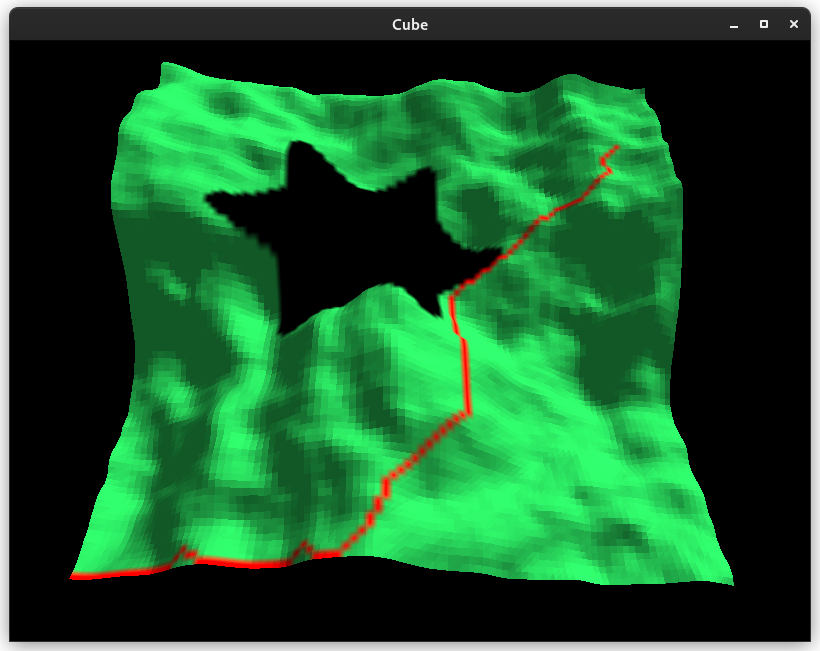
\includegraphics[scale=0.5]{content/bf-top.png}
    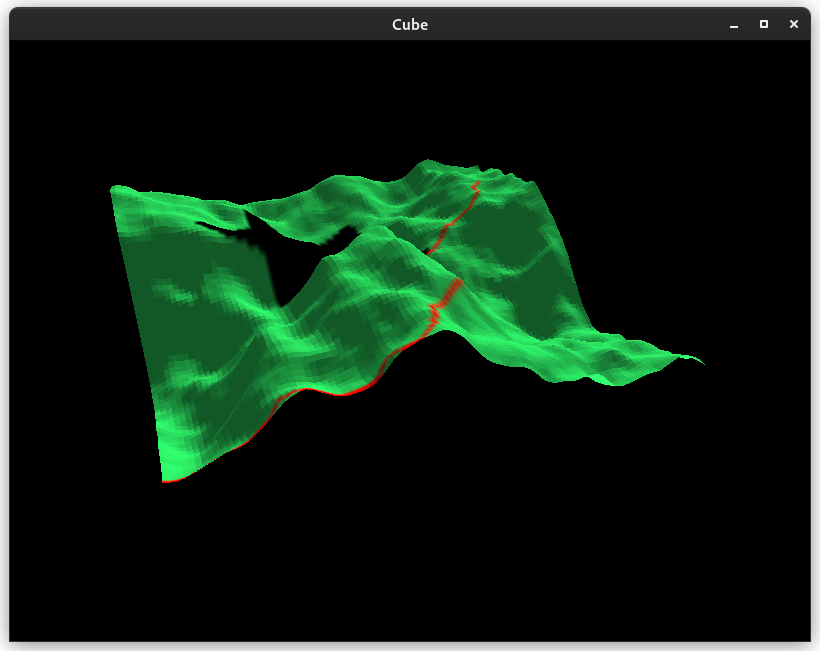
\includegraphics[scale=0.5]{content/bf.png}
    \caption{Результат работы алгоритма Беллмана--Форда на сетке 100$\times$100 c начальной позицией $(1, 1)$, конечной $(90, 90)$.}
\end{figure}
\clearpage
    \section{Сравнение алгоритмов}
    Ниже приведены времена работы различных версий программы в виде таблиц.
Интересно прослеживается закономерность нелинейного ускорения работы программы для алгоритма Дейкстры в связи с небольшим граничным множеством относительно размера сетки. Так же примерно виден процент времени передачи данных на многонодной установке, относительно времени вычислений.

Приложения запускались на ноутбуке автора с 8 ядерным процессором Intel® Core™ i7-6700HQ и 8 ГиБ ОЗУ.
Многонодная установка состояла из 3 виртуальных машин с 4 ядрами CPU и 8 ГиБ ОЗУ, две из которых использовались для вычислителей. Ноды были взяты у сервиса VK Cloud, который не предоставляет информацию об их физическом расположении и сетевой отдаленности.

\begin{figure}[h]
    \centering
    \begin{tabular}{ | l | l | l | l |}
        \hline
        Размер сетки & Классический & Парал. однонодный & Парал. многонодный \\ \hline
        50$\times$50 & & & \\
        100$\times$100 & 28s & 11s & \\
        250$\times$250 & & & \\
        500$\times$500 & & & \\
        \hline
    \end{tabular}
\caption{Время работы различных реализаций алгоритма Беллмана--Форда.}
\end{figure}

\begin{figure}[h]
    \centering
    \begin{tabular}{ | l | l | l | l |}
        \hline
        Размер сетки & Классический & Парал. однонодный & Парал. многонодный \\ \hline
        500$\times$500 & & & \\
        1000$\times$1000 & 36s & 40s & \\
        2500$\times$2500 & & & \\
        5000$\times$5000 & & & \\
        \hline
    \end{tabular}
    \caption{Время работы различных реализаций алгоритма Дейкстры.}
\end{figure}
    \newpage
    \section{Заключение}
    В рамках задачи на основе известных алгоритмов поиска кратчайшего пути в ориентированных графах были построены параллельные алгоритмы для решения задачи быстродействия при наличии фазовых ограничений.
Предложеные алгоритмы охватывают все степени параллелелизма, возможные на обычном компьюере: на ядрах центрального процессора, на графическом процессоре, на многоноднодной установке.

Также была выбрана архитектура и написана реализация параллельных алгоритмов Беллмана--Форда и Дейкстры на ядрах центрального процессора, и для многонодной установки.
Были проведены замеры времени работы различных алгоритмов на одинаковых начальных данных и схожем оборудовании для сравнения. Были описаны причины, приводящие к получившимся результатам.
    \newpage
    \begin{thebibliography}{9}
        \bibitem{bellman} Беллман~Р., Дрейфус~С. \textit{Прикладные задачи динамического программирования.} М.:~Наука,~1965.
        \bibitem{dijkstra} Shu-Xi, Wang. \textit{The Improved Dijkstra's Shortest Path Algorithm and Its Application.} Procedia Engineering. 29. 1186-1190. 2012.
        \bibitem{review} Glabowski, M., Musznicki, B., Nowak, P., Zwierzykowski, P. \textit{Review and Performance Analysis of Shortest Path Problem Solving Algorithms.} International Journal On Advances in Software. 7. 20-30. 2014.
        \bibitem{gyb} Корниенко~В.~С. \textit{Численные методы решения задач ``среднего поля''}:дис. к.ф.-м.н.: 05.13.18 --- Сибирский федеральный университет, Красноярск, 2021.
        \bibitem{optcontrol} Ведякова А. О., Милованович Е. В., Слита О. В., Тертычный-Даури В. Ю. \textit{Методы теории оптимального управления.} М.: Редакционно-издательский отдел Университета ИТМО. Санкт-Петербург, 2021.
        \bibitem{perlin} John Brosz, Faramarz F. Samavati and Mario Costa Sousa. \textit{Terrain Synthesis By-Example, Advances in Computer Graphics and Computer Vision.} Communications in Computer and Information Science 4, 2007, 58--77
    \end{thebibliography}
\end{document}


